\chapter{Background}
\label{ch:Background} 

%\section{RISC-V}
%
%\textbf{TODO: basic forklaring av RISC-V. Mulig det fra introdksjonen holder?}
%
%In RISC-V, the state of the processor is stored in multiple types of registers. The 32 \textit{general purpose registers (GPR)} are visible to the programmer in the unprivileged mode, are used for normal program execution, and are read and written to by the instructions \cite{waterman_risc-v_2019}. Additionally, the \textit{program counter (PC)} is the register that holds the address of the current instruction \cite{waterman_risc-v_2019}. There is also a set of registers that are typically inaccessible to the programmer in the unprivileged mode. These \textit{Control and Status Registers (CSR)} are used to control and monitor the operation of the processor.
%
%\section{Pipeline \& Interrupts}
%\label{sec:interrupts}

\section{RISC-V}

\tmp{Holder det som står i introduksjon?}

\section{Pipeline}
\label{sec:bg_pipeline}

Almost all of today's processor cores use pipelining to some extent to increase the throughput and reduce the cycle times of the processor. RISC-V has also been specifically designed for pipelined execution \cite{pattersonComputerOrganizationDesign2021}. 
Typically, a RISC-V pipeline has five steps \cite{pattersonComputerOrganizationDesign2021}:

\begin{itemize}
    \item \textbf{IF} - Fetch instructions from memory
    \item \textbf{ID} - Decode instruction and read registers
    \item \textbf{EX} - Execute the operation and calculate the memory address
    \item \textbf{MEM} - Read/write to the data memory
    \item \textbf{WB} - Write back the result from an operation to a register
\end{itemize}

\subsection{CV32E40S pipeline}
\label{sec:bg_cv32Pipeline}


\begin{figure}[htb]
    \centering
    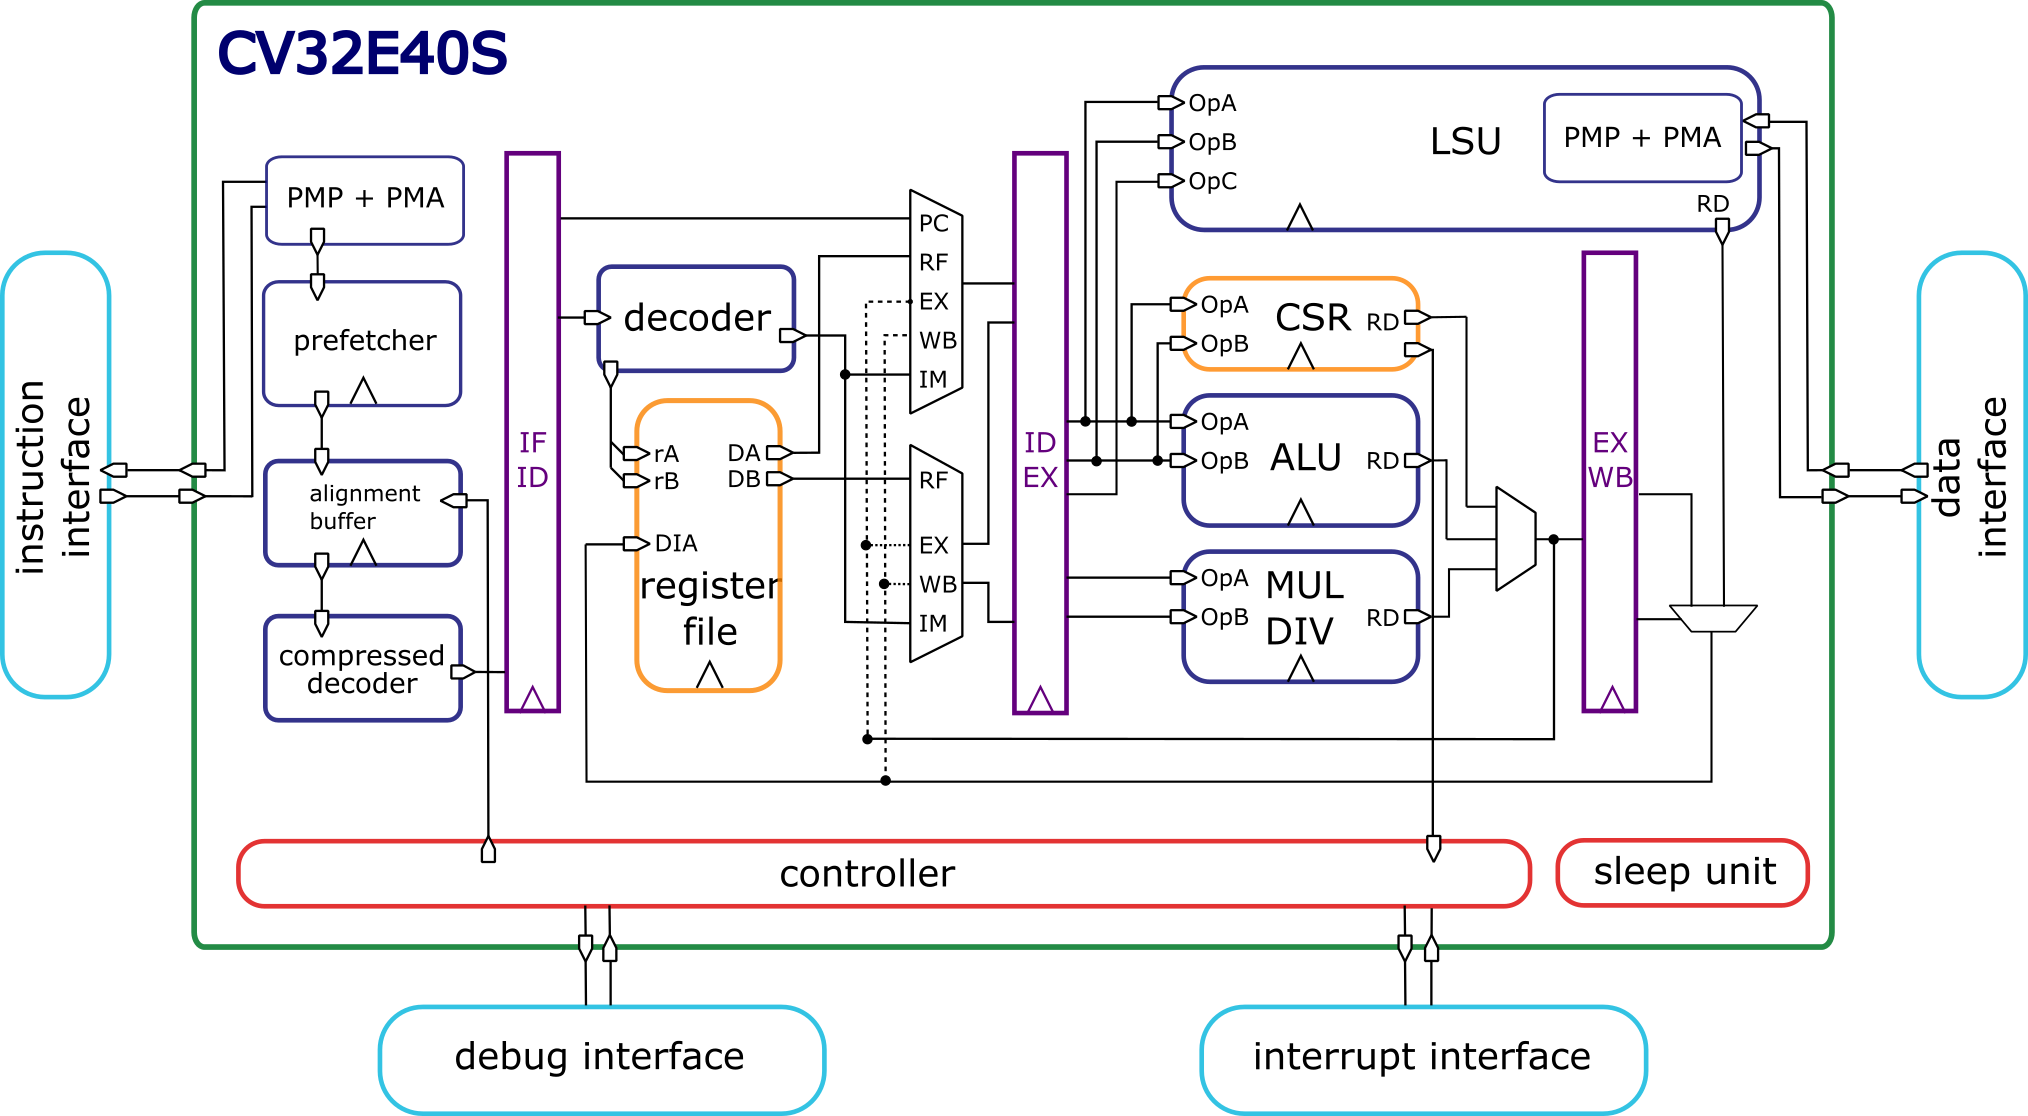
\includegraphics[width=\linewidth]{figures/CV32E40S_Block_Diagram.png}
    \caption{Block diagram of the CV32E40S RISC-V Core from \cite{openhwgroupIntroductionCOREVCV32E40S2023}.}
    \label{fig:cv32e40s-block}
\end{figure}

\Cref{fig:cv32e40s-block} shows a block diagram of the components and pipeline registers of the CV32E40S core from OpehHW Group.
The figure shows that the CV32E40S differs from the standard pipeline because it only has four pipeline stages. To achieve this, the \acrlong{lsu} responsible for loading and storing data from memory is divided so that the address generation is done in the EX stage, and the result is received in the WB stage.
The responsibilities of the four stages are explained below.

\subsubsection{Instruction Fetch (IF)}

The Program counter is increased, and the next instruction is fetched from memory through a prefetch buffer. This allows one instruction to be fetched per cycle if the memory allows it \cite{openhwgroupPipelineDetails2023}.

\subsubsection{Instruction Decode (ID)}

In the ID stage, the instruction is decoded, and the required registers are read from the register file. Additionally, jumps are initiated when a jump instruction arrives at the ID stage \cite{openhwgroupPipelineDetails2023}. 

\subsubsection{Execute (EX)}

The operation of an instruction is performed in the EX stage, such as ALU, multiplication, and division operations. Multi-cycle instructions, requiring multiple cycles to complete, cause the stage to be stalled until the operation is complete.

If the instruction contains a memory operation, the first phase of a memory read or write is initiated here. This involves generating the address to load or store to/from with with the corresponding control signals, and passing it to the \acrshort{lsu}.

Branches are also taken from the EX stage if their conditions are met \cite{openhwgroupPipelineDetails2023}

\subsubsection{Writeback (WB)}

In the WB stage, the results from the operation are written back to the register file. 
If the instruction contains a memory operation and was sent to the \acrshort{lsu} in the EX stage, the result from the \acrshort{lsu} is received and written back in the WB stage. If not, the result from the EX stage is written back to the register file \cite{openhwgroupPipelineDetails2023}.
We say that after an instruction has been written back in the WB stage, they are \gls{commited} or \gls{retired}, meaning that the instruction is fully executed and the effects of the instructions are executed \cite{taylorAdvancedRISCVVerification2023}. 


\subsubsection{Hazards \& Forwarding}

Because multiple instructions are in the pipeline simultaneously, \textit{Hazards} can arise where an instruction can not execute in the next clock cycle. Data hazards occur when there are dependencies between following instructions, where, for instance, the data needed in the ID stage by one instruction is written from the previous instruction, and the instruction has to wait until the previous instruction has written the data back to the register file in the WB stage.

\textit{Forwarding} attempts to solve this problem by allowing data to be forwarded to the stage that needs the data, avoiding stalls by not requiring the data to flow through the register file to a subsequent instruction.


\subsubsection{Side effects}

Most instructions follow a common pattern of reading values from registers, executing an operation, and returning the value to a register.
However, some instructions also have \textit{side effects}, which means that they update one or more state variables that are not directly a part of the instruction \cite{taylorAdvancedRISCVVerification2023}. This can, for instance, be changes to \acrshort{csr}s. For example \rv{mstatus} contains flags for different processors states 

\tmp{more on side effects (if it is necessary in background?)}

%Side effects in a RISC-V processor refer to any change in the state of the system that is not explicitly reflected in its return value. Side effects can include changes to memory, I/O devices, control and status registers, and more. Understanding side effects is essential for verifying the correctness of RISC-V processors and ensuring they behave as expected.
%
%One example of a side effect is the \lstinline{ecall} instruction, which triggers a software interrupt and transfers control to the operating system. The return value of the \lstinline{ecall} instruction is not relevant, but its side effect of transferring control to the OS is crucial.

\subsubsection{Flushing}

\glsdisp{flush}{Flushing} is when one or more pipeline stage must be discarded . This typically happens during exceptions, interrupts, branching, jumping, etc. where the fetched instructions differ from the instruction that should run next \cite{pattersonComputerOrganizationDesign2021}.

\Cref{fig:interrupt_flush} shows an example of the pipeline when an interrupt occurs. The figure shows the instructions contained in each pipeline stage for each clock cycle. In cycle 5 an interrupt occurs. In the next cycle, all the pipeline stages are flushed, ensuring that instruction 2 was the last instruction to be committed before taking the interrupt. In cycle 7, the pipeline starts to be filled up again, starting with the first instruction of the interrupt handler (IH1). We see that there is a 4-cycle delay between instruction 2 in cycle 5 and IH1 committing in cycle 10.

\Cref{fig:branch_flush} shows an example of the pipeline contents when a branch is taken. The figure shows that when the branch instruction (3 B) arrives in the EX stage in cycle 5, only the IF and ID stages are flushed, as they do not contain the correct instruction for the branch. This allows the first branch instruction (B1) to be fetched in cycle 6, while the branch instruction (3 B) is in the WB stage. Because of this, there is a 2-cycle delay where no instruction is committed in WB before the first instruction from the branch is committed.

\Cref{fig:jump_flush} shows a similar example with a flush instruction (3 J) instead of a branch instruction. Because branches are taken in the ID stage in the CV32E40S core, only the IF stage needs to be flushed and there is only one cycle delay before the first instruction after the jump.

\begin{figure}[htbp]
\centering
\begin{ganttchart}[
		x unit=1.4cm,
		y unit chart=0.7cm,
		canvas/.style={draw=none,fill=none}, % remove canvas borders, etc
		vgrid={*{2}{draw=black!8}},           % vertical gray lines every unit
		inline,                              % draw bars inline
		group/.style={draw=none,fill=none},  % remove group borders, etc
		bar top shift=0.1,                   % give bar 10% padding top/bottom
		bar height=0.8,                      % bar size 80% of vertical space
		y unit title=0.5cm,                  % crop titles a little smaller
		title/.style={draw=none,fill=none},  % remove title borders, etc
		include title in canvas=false        % no vertical grid in title
	]{0}{4}

    %\gantttitlelist{Cycle,IF,ID,EX,WB}{1}

	\gantttitle{Cycle}{-1}
	\gantttitle{IF}{3}
	\gantttitle{ID}{-1}
	\gantttitle{EX}{3}
	\gantttitle{WB}{-1} \\

	\ganttgroup[inline=false]{1}{0}{4}
	\ganttbar[bar/.style={draw=black!80,fill=orange!40}  ]{1}{0}{0}\\
 
	\ganttgroup[inline=false]{2}{0}{4}
	\ganttbar[bar/.style={draw=black!80,fill=yellow!40}  ]{2}{0}{0}
	\ganttbar[bar/.style={draw=black!80,fill=orange!40}  ]{1}{1}{1}\\
 
	\ganttgroup[inline=false]{3}{0}{4}
	\ganttbar[bar/.style={draw=black!80,fill=lime!40}    ]{3}{0}{0}
	\ganttbar[bar/.style={draw=black!80,fill=yellow!40}  ]{2}{1}{1}
	\ganttbar[bar/.style={draw=black!80,fill=orange!40}  ]{1}{2}{2}\\
 
	\ganttgroup[inline=false]{4}{0}{4}
	\ganttbar[bar/.style={draw=black!80,fill=green!40}   ]{4}{0}{0}
	\ganttbar[bar/.style={draw=black!80,fill=lime!40}    ]{3}{1}{1} 
	\ganttbar[bar/.style={draw=black!80,fill=yellow!40}  ]{2}{2}{2} 
	\ganttbar[bar/.style={draw=black!80,fill=orange!40}  ]{1}{3}{3} \\
 
	\ganttgroup[inline=false]{(IRQ) 5}{0}{4}
    \ganttbar[bar/.style={draw=black!80,fill=cyan!40}    ]{5}{0}{0} 
	\ganttbar[bar/.style={draw=black!80,fill=green!40}   ]{4}{1}{1}
	\ganttbar[bar/.style={draw=black!80,fill=lime!40}    ]{3}{2}{2} 
	\ganttbar[bar/.style={draw=black!80,fill=yellow!40}  ]{2}{3}{3}  \\


	\ganttgroup[inline=false]{(Flush) 6}{0}{1}
    \ganttbar[bar/.style={draw=black!80,fill=black!10}    ]{}{0}{0} 
    \ganttbar[bar/.style={draw=black!80,fill=black!10}    ]{}{1}{1} 
    \ganttbar[bar/.style={draw=black!80,fill=black!10}    ]{}{2}{2} 
    \ganttbar[bar/.style={draw=black!80,fill=black!10}    ]{}{3}{3} 
    
    \\
    
	\ganttgroup[inline=false]{7}{0}{1}
	\ganttbar[bar/.style={draw=black!80,fill=red!50}]{IH1}{0}{0} \\

	\ganttgroup[inline=false]{8}{0}{1}
	\ganttbar[bar/.style={draw=black!80,fill=orange!80}    ]{IH2}{0}{0}
	\ganttbar[bar/.style={draw=black!80,fill=red!50}       ]{IH1}{1}{1} \\
	
	\ganttgroup[inline=false]{9}{0}{1}
	\ganttbar[bar/.style={draw=black!80,fill=yellow!80}    ]{IH3}{0}{0}
	\ganttbar[bar/.style={draw=black!80,fill=orange!80}    ]{IH2}{1}{1}
	\ganttbar[bar/.style={draw=black!80,fill=red!50}       ]{IH1}{2}{2} \\
 
	\ganttgroup[inline=false]{10}{0}{1}
	\ganttbar[bar/.style={draw=black!80,fill=lime}       ]{IH4}{0}{0}
	\ganttbar[bar/.style={draw=black!80,fill=yellow!80}    ]{IH3}{1}{1}
	\ganttbar[bar/.style={draw=black!80,fill=orange!80}    ]{IH2}{2}{2}
	\ganttbar[bar/.style={draw=black!80,fill=red!50}       ]{IH1}{3}{3} \\


\end{ganttchart}
\caption{Pipeline flush during an interrupt.}
\label{fig:interrupt_flush}
\end{figure}

\begin{figure}[htbp]
\centering
\begin{ganttchart}[
		x unit=1.4cm,
		y unit chart=0.7cm,
		canvas/.style={draw=none,fill=none}, % remove canvas borders, etc
		vgrid={*{2}{draw=black!8}},           % vertical gray lines every unit
		inline,                              % draw bars inline
		group/.style={draw=none,fill=none},  % remove group borders, etc
		bar top shift=0.1,                   % give bar 10% padding top/bottom
		bar height=0.8,                      % bar size 80% of vertical space
		y unit title=0.5cm,                  % crop titles a little smaller
		title/.style={draw=none,fill=none},  % remove title borders, etc
		include title in canvas=false        % no vertical grid in title
	]{0}{4}

    %\gantttitlelist{Cycle,IF,ID,EX,WB}{1}

	\gantttitle{Cycle}{-1}
	\gantttitle{IF}{3}
	\gantttitle{ID}{-1}
	\gantttitle{EX}{3}
	\gantttitle{WB}{-1} \\

	\ganttgroup[inline=false]{1}{0}{4}
	\ganttbar[bar/.style={draw=black!80,fill=orange!40}  ]{1}{0}{0}\\
 
	\ganttgroup[inline=false]{2}{0}{4}
	\ganttbar[bar/.style={draw=black!80,fill=yellow!40}  ]{2}{0}{0}
	\ganttbar[bar/.style={draw=black!80,fill=orange!40}  ]{1}{1}{1}\\
 
	\ganttgroup[inline=false]{3}{0}{4}
	\ganttbar[bar/.style={draw=black!80,fill=lime!40}    ]{3 B}{0}{0}
	\ganttbar[bar/.style={draw=black!80,fill=yellow!40}  ]{2}{1}{1}
	\ganttbar[bar/.style={draw=black!80,fill=orange!40}  ]{1}{2}{2}\\
 
	\ganttgroup[inline=false]{4}{0}{4}
	\ganttbar[bar/.style={draw=black!80,fill=green!40}   ]{4}{0}{0}
	\ganttbar[bar/.style={draw=black!80,fill=lime!40}    ]{3 B}{1}{1} 
	\ganttbar[bar/.style={draw=black!80,fill=yellow!40}  ]{2}{2}{2} 
	\ganttbar[bar/.style={draw=black!80,fill=orange!40}  ]{1}{3}{3} \\
 
	\ganttgroup[inline=false]{(Flush) 5}{0}{4}
    \ganttbar[bar/.style={draw=black!80,fill=black!10}    ]{}{0}{0} 
    \ganttbar[bar/.style={draw=black!80,fill=black!10}    ]{}{1}{1} 
	\ganttbar[bar/.style={draw=black!80,fill=lime!40}    ]{3 B}{2}{2} 
	\ganttbar[bar/.style={draw=black!80,fill=yellow!40}  ]{2}{3}{3}  \\


	\ganttgroup[inline=false]{6}{0}{1}
	\ganttbar[bar/.style={draw=black!80,fill=red!50}]{B1}{0}{0}
	\ganttbar[bar/.style={draw=black!80,fill=lime!40}    ]{3 B}{3}{3} 
    \\
    
	\ganttgroup[inline=false]{7}{0}{1}
	\ganttbar[bar/.style={draw=black!80,fill=orange!80}    ]{B2}{0}{0}
	\ganttbar[bar/.style={draw=black!80,fill=red!50}       ]{B1}{1}{1} \\
	
	\ganttgroup[inline=false]{8}{0}{1}
	\ganttbar[bar/.style={draw=black!80,fill=yellow!80}    ]{B3}{0}{0}
	\ganttbar[bar/.style={draw=black!80,fill=orange!80}    ]{B2}{1}{1}
	\ganttbar[bar/.style={draw=black!80,fill=red!50}       ]{B1}{2}{2} \\
 
	\ganttgroup[inline=false]{9}{0}{1}
	\ganttbar[bar/.style={draw=black!80,fill=lime!80}      ]{B4}{0}{0}
	\ganttbar[bar/.style={draw=black!80,fill=yellow!80}    ]{B3}{1}{1}
	\ganttbar[bar/.style={draw=black!80,fill=orange!80}    ]{B2}{2}{2}
	\ganttbar[bar/.style={draw=black!80,fill=red!50}       ]{B1}{3}{3} \\


\end{ganttchart}
\caption{Pipeline flush during a branch.}
\label{fig:branch_flush}
\end{figure}

\begin{figure}[htbp]
\centering
\begin{ganttchart}[
		x unit=1.4cm,
		y unit chart=0.7cm,
		canvas/.style={draw=none,fill=none}, % remove canvas borders, etc
		vgrid={*{2}{draw=black!8}},           % vertical gray lines every unit
		inline,                              % draw bars inline
		group/.style={draw=none,fill=none},  % remove group borders, etc
		bar top shift=0.1,                   % give bar 10% padding top/bottom
		bar height=0.8,                      % bar size 80% of vertical space
		y unit title=0.5cm,                  % crop titles a little smaller
		title/.style={draw=none,fill=none},  % remove title borders, etc
		include title in canvas=false        % no vertical grid in title
	]{0}{4}

    %\gantttitlelist{Cycle,IF,ID,EX,WB}{1}

	\gantttitle{Cycle}{-1}
	\gantttitle{IF}{3}
	\gantttitle{ID}{-1}
	\gantttitle{EX}{3}
	\gantttitle{WB}{-1} \\

	\ganttgroup[inline=false]{1}{0}{4}
	\ganttbar[bar/.style={draw=black!80,fill=orange!40}  ]{1}{0}{0}\\
 
	\ganttgroup[inline=false]{2}{0}{4}
	\ganttbar[bar/.style={draw=black!80,fill=yellow!40}  ]{2}{0}{0}
	\ganttbar[bar/.style={draw=black!80,fill=orange!40}  ]{1}{1}{1}\\
 
	\ganttgroup[inline=false]{3}{0}{4}
	\ganttbar[bar/.style={draw=black!80,fill=lime!40}    ]{3 J}{0}{0}
	\ganttbar[bar/.style={draw=black!80,fill=yellow!40}  ]{2}{1}{1}
	\ganttbar[bar/.style={draw=black!80,fill=orange!40}  ]{1}{2}{2}\\
 
	\ganttgroup[inline=false]{(Flush) 4}{0}{4}
    \ganttbar[bar/.style={draw=black!80,fill=black!10}    ]{}{0}{0} 
	\ganttbar[bar/.style={draw=black!80,fill=lime!40}    ]{3 J}{1}{1} 
	\ganttbar[bar/.style={draw=black!80,fill=yellow!40}  ]{2}{2}{2} 
	\ganttbar[bar/.style={draw=black!80,fill=orange!40}  ]{1}{3}{3} \\
 
	\ganttgroup[inline=false]{5}{0}{4}
	\ganttbar[bar/.style={draw=black!80,fill=red!50}]{B1}{0}{0}
	\ganttbar[bar/.style={draw=black!80,fill=lime!40}    ]{3 J}{2}{2} 
	\ganttbar[bar/.style={draw=black!80,fill=yellow!40}  ]{2}{3}{3}  \\


	\ganttgroup[inline=false]{6}{0}{1}
	\ganttbar[bar/.style={draw=black!80,fill=orange!80}    ]{B2}{0}{0}
	\ganttbar[bar/.style={draw=black!80,fill=red!50}       ]{B1}{1}{1}
	\ganttbar[bar/.style={draw=black!80,fill=lime!40}    ]{3 J}{3}{3} 
    \\
    
	\ganttgroup[inline=false]{7}{0}{1}
	\ganttbar[bar/.style={draw=black!80,fill=yellow!80}    ]{B3}{0}{0}
	\ganttbar[bar/.style={draw=black!80,fill=orange!80}    ]{B2}{1}{1}
	\ganttbar[bar/.style={draw=black!80,fill=red!50}       ]{B1}{2}{2} \\
	
	\ganttgroup[inline=false]{8}{0}{1}
	\ganttbar[bar/.style={draw=black!80,fill=lime!80}      ]{B4}{0}{0}
	\ganttbar[bar/.style={draw=black!80,fill=yellow!80}    ]{B3}{1}{1}
	\ganttbar[bar/.style={draw=black!80,fill=orange!80}    ]{B2}{2}{2}
	\ganttbar[bar/.style={draw=black!80,fill=red!50}       ]{B1}{3}{3} \\


\end{ganttchart}
\caption{Pipeline flush during a jump.}
\label{fig:jump_flush}
\end{figure}


%\begin{figure}
%    \centering
%    \begin{subfigure}[b]{.3\textwidth}
%        \centering
%        \resizebox{1.2\columnwidth}{!}{
%            \begin{ganttchart}[
		x unit=1.4cm,
		y unit chart=0.7cm,
		canvas/.style={draw=none,fill=none}, % remove canvas borders, etc
		vgrid={*{2}{draw=black!8}},           % vertical gray lines every unit
		inline,                              % draw bars inline
		group/.style={draw=none,fill=none},  % remove group borders, etc
		bar top shift=0.1,                   % give bar 10% padding top/bottom
		bar height=0.8,                      % bar size 80% of vertical space
		y unit title=0.5cm,                  % crop titles a little smaller
		title/.style={draw=none,fill=none},  % remove title borders, etc
		include title in canvas=false        % no vertical grid in title
	]{0}{4}

    %\gantttitlelist{Cycle,IF,ID,EX,WB}{1}

	\gantttitle{Cycle}{-1}
	\gantttitle{IF}{3}
	\gantttitle{ID}{-1}
	\gantttitle{EX}{3}
	\gantttitle{WB}{-1} \\

	\ganttgroup[inline=false]{1}{0}{4}
	\ganttbar[bar/.style={draw=black!80,fill=orange!40}  ]{1}{0}{0}\\
 
	\ganttgroup[inline=false]{2}{0}{4}
	\ganttbar[bar/.style={draw=black!80,fill=yellow!40}  ]{2}{0}{0}
	\ganttbar[bar/.style={draw=black!80,fill=orange!40}  ]{1}{1}{1}\\
 
	\ganttgroup[inline=false]{3}{0}{4}
	\ganttbar[bar/.style={draw=black!80,fill=lime!40}    ]{3}{0}{0}
	\ganttbar[bar/.style={draw=black!80,fill=yellow!40}  ]{2}{1}{1}
	\ganttbar[bar/.style={draw=black!80,fill=orange!40}  ]{1}{2}{2}\\
 
	\ganttgroup[inline=false]{4}{0}{4}
	\ganttbar[bar/.style={draw=black!80,fill=green!40}   ]{4}{0}{0}
	\ganttbar[bar/.style={draw=black!80,fill=lime!40}    ]{3}{1}{1} 
	\ganttbar[bar/.style={draw=black!80,fill=yellow!40}  ]{2}{2}{2} 
	\ganttbar[bar/.style={draw=black!80,fill=orange!40}  ]{1}{3}{3} \\
 
	\ganttgroup[inline=false]{(IRQ) 5}{0}{4}
    \ganttbar[bar/.style={draw=black!80,fill=cyan!40}    ]{5}{0}{0} 
	\ganttbar[bar/.style={draw=black!80,fill=green!40}   ]{4}{1}{1}
	\ganttbar[bar/.style={draw=black!80,fill=lime!40}    ]{3}{2}{2} 
	\ganttbar[bar/.style={draw=black!80,fill=yellow!40}  ]{2}{3}{3}  \\


	\ganttgroup[inline=false]{(Flush) 6}{0}{1}
    \ganttbar[bar/.style={draw=black!80,fill=black!10}    ]{}{0}{0} 
    \ganttbar[bar/.style={draw=black!80,fill=black!10}    ]{}{1}{1} 
    \ganttbar[bar/.style={draw=black!80,fill=black!10}    ]{}{2}{2} 
    \ganttbar[bar/.style={draw=black!80,fill=black!10}    ]{}{3}{3} 
    
    \\
    
	\ganttgroup[inline=false]{7}{0}{1}
	\ganttbar[bar/.style={draw=black!80,fill=red!50}]{IH1}{0}{0} \\

	\ganttgroup[inline=false]{8}{0}{1}
	\ganttbar[bar/.style={draw=black!80,fill=orange!80}    ]{IH2}{0}{0}
	\ganttbar[bar/.style={draw=black!80,fill=red!50}       ]{IH1}{1}{1} \\
	
	\ganttgroup[inline=false]{9}{0}{1}
	\ganttbar[bar/.style={draw=black!80,fill=yellow!80}    ]{IH3}{0}{0}
	\ganttbar[bar/.style={draw=black!80,fill=orange!80}    ]{IH2}{1}{1}
	\ganttbar[bar/.style={draw=black!80,fill=red!50}       ]{IH1}{2}{2} \\
 
	\ganttgroup[inline=false]{10}{0}{1}
	\ganttbar[bar/.style={draw=black!80,fill=lime}       ]{IH4}{0}{0}
	\ganttbar[bar/.style={draw=black!80,fill=yellow!80}    ]{IH3}{1}{1}
	\ganttbar[bar/.style={draw=black!80,fill=orange!80}    ]{IH2}{2}{2}
	\ganttbar[bar/.style={draw=black!80,fill=red!50}       ]{IH1}{3}{3} \\


\end{ganttchart}
%        }
%        \caption{Pipeline flush during an interrupt.}
%        \label{fig:interrupt_flush}
%        
%    \end{subfigure}
%    \hfill
%    \begin{subfigure}[b]{.3\textwidth}
%        \centering
%        \resizebox{1.2\columnwidth}{!}{
%            \begin{ganttchart}[
		x unit=1.4cm,
		y unit chart=0.7cm,
		canvas/.style={draw=none,fill=none}, % remove canvas borders, etc
		vgrid={*{2}{draw=black!8}},           % vertical gray lines every unit
		inline,                              % draw bars inline
		group/.style={draw=none,fill=none},  % remove group borders, etc
		bar top shift=0.1,                   % give bar 10% padding top/bottom
		bar height=0.8,                      % bar size 80% of vertical space
		y unit title=0.5cm,                  % crop titles a little smaller
		title/.style={draw=none,fill=none},  % remove title borders, etc
		include title in canvas=false        % no vertical grid in title
	]{0}{4}

    %\gantttitlelist{Cycle,IF,ID,EX,WB}{1}

	\gantttitle{Cycle}{-1}
	\gantttitle{IF}{3}
	\gantttitle{ID}{-1}
	\gantttitle{EX}{3}
	\gantttitle{WB}{-1} \\

	\ganttgroup[inline=false]{1}{0}{4}
	\ganttbar[bar/.style={draw=black!80,fill=orange!40}  ]{1}{0}{0}\\
 
	\ganttgroup[inline=false]{2}{0}{4}
	\ganttbar[bar/.style={draw=black!80,fill=yellow!40}  ]{2}{0}{0}
	\ganttbar[bar/.style={draw=black!80,fill=orange!40}  ]{1}{1}{1}\\
 
	\ganttgroup[inline=false]{3}{0}{4}
	\ganttbar[bar/.style={draw=black!80,fill=lime!40}    ]{3 B}{0}{0}
	\ganttbar[bar/.style={draw=black!80,fill=yellow!40}  ]{2}{1}{1}
	\ganttbar[bar/.style={draw=black!80,fill=orange!40}  ]{1}{2}{2}\\
 
	\ganttgroup[inline=false]{4}{0}{4}
	\ganttbar[bar/.style={draw=black!80,fill=green!40}   ]{4}{0}{0}
	\ganttbar[bar/.style={draw=black!80,fill=lime!40}    ]{3 B}{1}{1} 
	\ganttbar[bar/.style={draw=black!80,fill=yellow!40}  ]{2}{2}{2} 
	\ganttbar[bar/.style={draw=black!80,fill=orange!40}  ]{1}{3}{3} \\
 
	\ganttgroup[inline=false]{(Flush) 5}{0}{4}
    \ganttbar[bar/.style={draw=black!80,fill=black!10}    ]{}{0}{0} 
    \ganttbar[bar/.style={draw=black!80,fill=black!10}    ]{}{1}{1} 
	\ganttbar[bar/.style={draw=black!80,fill=lime!40}    ]{3 B}{2}{2} 
	\ganttbar[bar/.style={draw=black!80,fill=yellow!40}  ]{2}{3}{3}  \\


	\ganttgroup[inline=false]{6}{0}{1}
	\ganttbar[bar/.style={draw=black!80,fill=red!50}]{B1}{0}{0}
	\ganttbar[bar/.style={draw=black!80,fill=lime!40}    ]{3 B}{3}{3} 
    \\
    
	\ganttgroup[inline=false]{7}{0}{1}
	\ganttbar[bar/.style={draw=black!80,fill=orange!80}    ]{B2}{0}{0}
	\ganttbar[bar/.style={draw=black!80,fill=red!50}       ]{B1}{1}{1} \\
	
	\ganttgroup[inline=false]{8}{0}{1}
	\ganttbar[bar/.style={draw=black!80,fill=yellow!80}    ]{B3}{0}{0}
	\ganttbar[bar/.style={draw=black!80,fill=orange!80}    ]{B2}{1}{1}
	\ganttbar[bar/.style={draw=black!80,fill=red!50}       ]{B1}{2}{2} \\
 
	\ganttgroup[inline=false]{9}{0}{1}
	\ganttbar[bar/.style={draw=black!80,fill=lime!80}      ]{B4}{0}{0}
	\ganttbar[bar/.style={draw=black!80,fill=yellow!80}    ]{B3}{1}{1}
	\ganttbar[bar/.style={draw=black!80,fill=orange!80}    ]{B2}{2}{2}
	\ganttbar[bar/.style={draw=black!80,fill=red!50}       ]{B1}{3}{3} \\


\end{ganttchart}
%        }
%        \caption{Pipeline flush during a branch.}
%        \label{fig:branch_flush}
%    \end{subfigure}
%    \begin{subfigure}[b]{.3\textwidth}
%        \centering
%        \resizebox{1.2\columnwidth}{!}{
%            \begin{ganttchart}[
		x unit=1.4cm,
		y unit chart=0.7cm,
		canvas/.style={draw=none,fill=none}, % remove canvas borders, etc
		vgrid={*{2}{draw=black!8}},           % vertical gray lines every unit
		inline,                              % draw bars inline
		group/.style={draw=none,fill=none},  % remove group borders, etc
		bar top shift=0.1,                   % give bar 10% padding top/bottom
		bar height=0.8,                      % bar size 80% of vertical space
		y unit title=0.5cm,                  % crop titles a little smaller
		title/.style={draw=none,fill=none},  % remove title borders, etc
		include title in canvas=false        % no vertical grid in title
	]{0}{4}

    %\gantttitlelist{Cycle,IF,ID,EX,WB}{1}

	\gantttitle{Cycle}{-1}
	\gantttitle{IF}{3}
	\gantttitle{ID}{-1}
	\gantttitle{EX}{3}
	\gantttitle{WB}{-1} \\

	\ganttgroup[inline=false]{1}{0}{4}
	\ganttbar[bar/.style={draw=black!80,fill=orange!40}  ]{1}{0}{0}\\
 
	\ganttgroup[inline=false]{2}{0}{4}
	\ganttbar[bar/.style={draw=black!80,fill=yellow!40}  ]{2}{0}{0}
	\ganttbar[bar/.style={draw=black!80,fill=orange!40}  ]{1}{1}{1}\\
 
	\ganttgroup[inline=false]{3}{0}{4}
	\ganttbar[bar/.style={draw=black!80,fill=lime!40}    ]{3 J}{0}{0}
	\ganttbar[bar/.style={draw=black!80,fill=yellow!40}  ]{2}{1}{1}
	\ganttbar[bar/.style={draw=black!80,fill=orange!40}  ]{1}{2}{2}\\
 
	\ganttgroup[inline=false]{(Flush) 4}{0}{4}
    \ganttbar[bar/.style={draw=black!80,fill=black!10}    ]{}{0}{0} 
	\ganttbar[bar/.style={draw=black!80,fill=lime!40}    ]{3 J}{1}{1} 
	\ganttbar[bar/.style={draw=black!80,fill=yellow!40}  ]{2}{2}{2} 
	\ganttbar[bar/.style={draw=black!80,fill=orange!40}  ]{1}{3}{3} \\
 
	\ganttgroup[inline=false]{5}{0}{4}
	\ganttbar[bar/.style={draw=black!80,fill=red!50}]{B1}{0}{0}
	\ganttbar[bar/.style={draw=black!80,fill=lime!40}    ]{3 J}{2}{2} 
	\ganttbar[bar/.style={draw=black!80,fill=yellow!40}  ]{2}{3}{3}  \\


	\ganttgroup[inline=false]{6}{0}{1}
	\ganttbar[bar/.style={draw=black!80,fill=orange!80}    ]{B2}{0}{0}
	\ganttbar[bar/.style={draw=black!80,fill=red!50}       ]{B1}{1}{1}
	\ganttbar[bar/.style={draw=black!80,fill=lime!40}    ]{3 J}{3}{3} 
    \\
    
	\ganttgroup[inline=false]{7}{0}{1}
	\ganttbar[bar/.style={draw=black!80,fill=yellow!80}    ]{B3}{0}{0}
	\ganttbar[bar/.style={draw=black!80,fill=orange!80}    ]{B2}{1}{1}
	\ganttbar[bar/.style={draw=black!80,fill=red!50}       ]{B1}{2}{2} \\
	
	\ganttgroup[inline=false]{8}{0}{1}
	\ganttbar[bar/.style={draw=black!80,fill=lime!80}      ]{B4}{0}{0}
	\ganttbar[bar/.style={draw=black!80,fill=yellow!80}    ]{B3}{1}{1}
	\ganttbar[bar/.style={draw=black!80,fill=orange!80}    ]{B2}{2}{2}
	\ganttbar[bar/.style={draw=black!80,fill=red!50}       ]{B1}{3}{3} \\


\end{ganttchart}
%        }
%        \caption{Pipeline flush during a jump.}
%        \label{fig:jump_flush}
%    \end{subfigure}
%    
%    \caption{A figure composed of two sub-figures. It has a long caption in order to demonstrate how that is typeset.}
%    \label{fig:subfig}
%\end{figure}



\section{Interrupts}
\label{sec:bg_interrupts}

In the RISC-V specification, there is a distinction between interrupts and exceptions. An \textit{interrupt} is an external event that occurs asynchronously to the execution, whereas an \textit{exception} is an unusual condition associated with an instruction at run time, happening synchronously to the execution. In RISC-V, a \textit{trap} can be triggered by both an interrupt and exception, leading to the transfer of control to a \textit{trap handler}. A trap handler is a set of specialized instructions to manage the exception or interrupt appropriately \cite{watermanRISCVInstructionSet2021}. 

An \textit{asynchronous event} can either be an external interrupt or a debug request. This event happens independently of the normal program flow and clock cycle. In the report, we will mostly focus on interrupts as examples of asynchronous events, but many of the same timing problems presented will also apply to debug requests.


The CV32E40S supports two different interrupt architectures, the simpler, non-preemptable \acrfull{clint} and the more sophisticated \acrfull{clic}, which supports nested interrupts with interrupt prioritization, and a larger number of interrupts \cite{openhwgroupExceptionsInterruptsCOREV2023}. 


To simplify the explanation, we will focus on the CLINT implementation as an example of how interrupts are handled. However, we will also briefly discuss the differences between CLINT and CLIC. 

\subsubsection{CLINT}
Interrupts are communicated to the core through the control and status registers (CSRs).

When an interrupt is detected by the CLINT, either from a peripheral or software, the bit corresponding to the interrupt is set in the interrupt pending register, \lstinline{mip}, signaling that the interrupt is pending.
Interrupts can be disabled and enabled using the interrupt enable register, \lstinline{mie}, which is checked against \lstinline{mip}. All interrupts for a given privilege level can also be disabled and enabled using the \lstinline{mstatus.mie} CSR. An interrupt is considered enabled when \lstinline{mstatus.mie} is enabled, and the interrupt bit is set in both \lstinline{mip} and \lstinline{mie} \cite{watermanRISCVInstructionSet2021}.

When an interrupt is enabled, the processor can \textit{take} the interrupt, causing the following to be done:

The current PC is captured into the \lstinline{mepc} CSR to continue the interrupted program after the interrupt execution. 
The interrupt cause is saved into the \lstinline{mcause} register, which the trap handler uses to determine the correct handling.
Since CLINT is non-preemptive, the core disables interrupts while in the trap handler by clearing the \lstinline{mstatus.mie} register, after saving the previous state to \lstinline{mstatus.mpie} to be able to revert it afterwards. 
The interrupts handler is looked up in the vector table \lstinline{mtvec}, and this base address is jumped to if non-vectored mode is enabled, or if vectored mode is enabled, the core jumps to the base address plus an offset address of 4 times the interrupt ID. This requires \textit{flushing} the pipeline, discarding the unfinished instructions.


The interrupt handler ends with the \lstinline{mret} instruction, which reverts the program counter to the PC saved in \lstinline{mepc}, and reverts \lstinline{mstatus.mie} from \lstinline{mstatus.mpie}.

\subsection{Non-Maskable interrupts - NMI}

Non-maskable Interrupts are used only for hardware errors. They can not be disabled and perform a jump to the NMI vector to be handled \cite{watermanRISCVInstructionSet2021}. They update \lstinline{mepc}, \lstinline{mcause}, and \lstinline{mstatus} like normal interrupts, but NMIs are handled in an imprecise manner, allowing the instruction causing the NMI to retire before taking the NMI. At most, two instructions will retire before NMI is taken. 
Additionally, NMIs have a higher priority than other interrupts and will be taken before other pending interrupts. \cite{openhwgroupExceptionsInterruptsCOREV2023}

\subsection{CLIC}

The \textit{Core Local Interrupt Controller (CLIC)} is a more advanced interrupt controller, supporting priority levels of interrupt, nestable interrupts, and up to 4096 interrupts (1024 in CV32E40S) \cite{openhwgroupExceptionsInterruptsCOREV2023}. CLIC's functionality is somewhat different to CLINT's explained above, but the differences are not essential to understanding the complexity of verifying interrupts and will not be discussed further. 

\subsection{Consequence of interrupts in the pipeline}

The pipeline state can affect the timing of interrupts. When an interrupt occurs, the processor must halt normal execution at the current instruction and switch to the interrupt handler. When the core takes the interrupt and jumps to the interrupt handler, the pipeline stages must be flushed or killed. This involves discarding the unfinished instructions currently in the pipeline. However, the pipeline may not always be in a state where it can be safely flushed. This can occur in multiple scenarios, such as if the processor is mid-execution of a multi-cycle instruction or has an outstanding memory operation. This requires the core to wait for the pipeline to be \textit{interruptible} before taking the interrupt \cite{taylorAdvancedRISCVVerification2023}.





\tmp{Forklar med \Cref{fig:interrupt_flush}}

\section{Debug requests}
\label{sec:bg_debug}

Debug support is an essential part of a processor, to allow developers to gain visibility and control of the processor, especially when implemented physically in hardware. CV32E40S supports the RISC-V Debug Specification \cite{pauldonahueRISCVDebugSupport2023} to support low level debugging access to the processor. The specification defines a common interface used by \acrfull{dm} on the RISC-V platform, but external to the core. This \acrshort{dm} is further controlled by a Debugger on a Debug Host (eg. gdb on a laptop), through Debug Transport Hardware (eg. JTAG), and through different transport modules and interfaces. 

The Debug Mode of the core can be entered synchronously through \rv{ebreak} instructions, or asynchronously through the \rv{debug_req_i} input signal to the core used by the \acrshort{dm} \cite{openhwgroupDebugTriggerCOREV2023}.

When the core enters the the debug mode, the current PC is saved to the \rv{dpc} CSR, the cause of the debug is saved in the \rv{dcsr} CSR, and the privilege is set in \rv{prv}. The PC is then redirected to a location given in the \rv{dm_haltaddr_i} port, where the processor starts executing the debug control code from \cite{openhwgroupDebugTriggerCOREV2023}.

To exit from debug mode, the \rv{dret} instruction is executed, which restores the PC from \rv{dpc} and resumes normal execution at the privilege level set in \rv{prv} and \rv{v} \cite{pauldonahueRISCVDebugSupport2023}.

\section{Processor verification Techniques}
\label{sec:bg_verificationTech}

%\textbf{TODO: Compliance vs DV}

A common approach to processor verification is the \textit{step-and-compare} methodology \cite{taylorAdvancedRISCVVerification2023}. Here, the \textit{Device Under Test (DUT)} RTL code runs parallel to a Reference Model (RM) in the testbench. They run in \textit{lock-step}, executing the same instructions from a random instruction stream generator, and the state of the DUT and RM is compared after each instruction \textit{retires}. An instruction has retired when the execution of the instruction has been completed, and all the values of the \textit{program counter (PC)}, \textit{General Purpose Registers (GPRs)}, and \textit{Control and Status Registers (CSRs)} are updated \cite{taylorAdvancedRISCVVerification2023}. These signals are output at retirement through a tracer like RVFI, as explained in \cref{sec:rvfi}.

\subsection{step-and-compare}
\label{sec:step-and-compare}
The step-and-compare methodology is popular since the state is continuously compared between the DUT and the RM, and there are no wasted cycles after a failure. This is an advantage compared to other methodologies such as post-simulation trace log checking and post-simulation signature checking \cite{duncangrahamRISCVVerificationImplications2023}, where the program has to fully complete before comparing the logs and determining if the test has passed or failed.

\section{Instruction Set Simulators (ISS) }
\label{sec:bg_iss}

An \textit{Instruction Set Simulator (ISS)} is a simulator that simulates the processor execution at an instruction granularity.
It only takes the ISA as a basis and ignores implementation-specifics like the pipeline.
There are many available Instruction Set Simulators for RISC-V, some of which are discussed below.

%\subsection{QEMU}
%\label{sec:qemu}
%
%\textit{QEMU} is an open-source full-system emulator that can run various operating systems on multiple hardware platforms. It supports multiple ISAs, one of which is RISC-V \cite{qemu_project_developers_about_2023}. 
%It uses portable dynamic binary translation to translate full code blocks from one another ISA to RISC-V. QEMU is made to be fast, and multiple optimizations and simplifications are made at the expense of accuracy. For instance, interrupts are not checked at every instruction but at every new code block, so interrupts may be mistimed. \cite{bellard_qemu_2005}
%
%\subsection{Rv8}
%\label{sec:rv8}
%
%\textit{Rv8} is another open-source ISS that uses just-in-time dynamic binary translation, similar to QEMU. Like QEMU, it is also focused on speed, does optimizations at the expense of accuracy, and may be hard to use for verification \cite{clark_rv8_2017}.
%
%\subsection{R2VM}
%\label{sec:R2VM}
%
%The \textit{Rust RISC-V Virtual Machine (R2VM)} \cite{guo_accelerate_2020} is an ISS written in Rust. It utilizes \textit{dynamic binary translation (DBT)} to translate code blocks from the RISC-V ISA to the host's native code. 
%
%The simulator also simulates a 5-stage pipeline. This implementation models the pipeline during the DBT code generation and uses different "hooks" that run at the start of a block, before an instruction, after an instruction, and after a taken branch. The hooks generate microarchitectural simulation code and are used to calculate the number of cycles it takes for an instruction to complete. 
%
%Because the simulator uses DBT, interrupts are checked only at the end of basic blocks since it is difficult to interrupt DBT-ed code \cite{guo_accelerate_2020}. This can be accepted in the R2VM simulator as it is intended for simulating timing, but is not optimal for verification.
%
%
%
%\subsection{riscvOVPsim}
%\label{sec:riscvOVPsim}
%
%\textit{riscvOVPsim} is a free ISS from Imperas. Imperas is a leading processor simulation company. It is instruction-accurate with support for most official RISC-V extensions. It allows configuring the model with different configurations and standard extensions, but riscvOVPsim only works with the standard RISC-V extensions and does not allow users to add custom instructions and extensions without acquiring a license from Imperas. \cite{imperas_software_ltd_risc-v_2023}.
%
%\textit{riscvOVPsimPlus} is an expanded version of riscvOVPsim that adds trace output and a GDB debug interface. It allows an execution log to be output and compared after execution. \cite{imperas_software_ltd_risc-v_2023}

\subsection{Spike}
\label{sec:spike}

\textit{Spike} is an open-source functional instruction-accurate ISS written for RISC-V. It is written in C++ and is relatively simple to use and extend. It is widely used in both academia for research and teaching, and in industry as a golden functional reference to multiple RISC-V cores. Spike is the official RISC-V ISS developed alongside the RISC-V specification as the golden model since 2010 and is now maintained by RISC-V International. \cite{SpikeRISCVISA2023}

Spike supports a wide variety of extensions and makes it relatively simple to include custom extensions.
The widespread adoption of Spike is a big advantage as it has been thoroughly tested, leaving few bugs, and is likely to be kept up-to-date for the foreseeable future. 

Spike loads in an ELF binary file holding the instructions to be run.
\tmp{More on how spike works?}
%Spike revolves around a \lstinline{step()} function in the \lstinline{execute.cc} file that fetches, decodes, and executes an instruction. This is divided into one function \lstinline{_mmu->access_icache(pc)} that fetches an already decoded instruction (with \lstinline{decode()}) with the type \lstinline{insn_fetch_t}, and either run \lstinline{execute_insn_fast()} or \lstinline{execute_insn_logged()} to execute the instruction quickly or slowly with logging. In Spike, the execute functions also write the results to the simulated register file \cite{SpikeRISCVISA2023}.

\subsection{Sail-riscv}
\label{sec:sail}

\textit{Sail-riscv} is a model of RISC-V written in the Sail language. Sail is a language specifically for specifying instruction set architectures for a processor. It is intended as being a precise definition of the ISA to avoid ambiguity of an ISA specification written in text or pseudocode \cite{armstrongSailInstructionsetSemantics2023}. It features an OCaml parser and backend, allowing the generation of latex documentation, executable emulators in C and OCaml, theorem prover definitions, and type checking. 

Sail-riscv is the sail specification for RISC-V and has been adopted as the golden formal model by the RISC-V Foundation\cite{RISCVSailModel2023}. 
The C-emulator generated from the sail-riscv model makes it possible to use the model as an ISS. The emulator mixes autogenerated code from the sail model with handwritten wrapper code. The generator can be configured to use different extensions, and custom extensions written in Sail can also be included in the simulator. 

Sail-riscv also revolves around a \lstinline{step()} function. Inside the step function, instructions are fetched with the \lstinline{fetch()} function, decoded with \lstinline{ext_decode()}, and executed with \lstinline{execute()}. Execute also writes the data back to the register file and executes side effects. \cite{RISCVSailModel2023}


%\begin{itemize}
%  \item Emulator generated from the risc-v sail specification.
%  \item the c emulator is an interpreter. Fetches and decodes instructions from emulated ram. \cite{}
%  \item Supports RVFI\_DII (Risc-V Formal Interface - Direct Instruction Injection)
%  \item Supports RV32I, RV64I, M, A, C, F, D, Zicsr and N extensions
%  \item \textbf{Lacking} support for multiple extensions: E, Zmmul, Zicntr, Zihpm, Zifencei... 
%  \item openHW has been considering implementing these in sail \textbf{but unclear what the status is}. 
%  \item base counters and timers
%  \item Machine-level and supervisor-level
%  \item supports CLINT
%\end{itemize}


%\section{Micro-Architectural simulators}
%
%Micro-architectural simulators simulate computer systems by modeling the different underlying hardware components, achieving cycle-accurate simulation \cite{akram_survey_2019}. Some micro-architectural simulators will be introduced below.
%
%
%\subsection{Gem5}
%\label{sec:gem5}
%
%\textit{Gem5} is an open-source architecture simulator. It decouples the ISA semantics from the CPU model, allowing the simulation of multiple ISAs and CPU models. It has support for atomic, in-order, and out-of-order CPU models, and recently received support for RISC-V \cite{roelke_risc5_2017} \cite{hin_supporting_2021} \cite{lowe-power_gem5_2020}. 
%
%Gem5 is popular for architectural exploration but lacks some features that might be necessary for verification. For example, it lacks support for running in lock-step execution, lacks a trace output for each cycle, and is non-trivial to add custom instructions and extensions.
%
%While Gem5 is cycle-accurate, significant modifications to the included prebuilt CPU models are necessary to represent the DUT core accurately. 
%
%Gem5 is actively developed and maintained and is likely to continue getting support. \cite{noauthor_gem5_2023}
%
%%\begin{itemize}
%%    \item Open source architecture simulator
%%    \item Hardware is black boxes with tunable latencies and attributes
%%    \item Multiple CPU models; atomic, in-order, out-of-order
%%    \item Decouples ISA semantics from the CPU models
%%    \item Might be slow compared to other ISS alternatives
%%    \item Syscall Emulation (SE) mode simulation or Full System (FS) mode simulation
%%\end{itemize}
%%
%%Gem5 is intended for performance evaluation, so to use it for validation, some work has to be done.
%%We need to support:
%%
%%\begin{itemize}
%%    \item Lock-step execution
%%    \item trace output for each cycle
%%    \item Ability to supoprt custom extensions and instructions
%%    \item Modify the cpu model to resemble the core to be simulated.
%%    \item Modularity in choosing RISC-V extensions
%%\end{itemize}
%
%%Gem5 is more complex than spike and sail, but might be harder to modify without altering side effects
%%
%%Gem5 might lead to more work to modify and/or might be more messy.
%%
%%Could become too similar to the RTL, and possibly have the same bugs.
%
%
%%\subsection{TinyEMU}
%%
%%\begin{itemize}
%%    \item System emulator
%%    \item Small and simple
%%\end{itemize}
%
%\subsection{MARSS-RISCV}
%\label{sec:marss}
%
%\textit{MARSS-RISCV} is an open-source cycle-level micro-architectural simulator for RISC-V, built on top of the TinyEMU emulator. It has cycle-level models for both in-order and out-of-order pipelines, configurable with 5-stage- and 6-stage pipelines \cite{kothari_marss-riscv_2019}. It is also intended for full system simulation, performance evaluation, or architectural exploration, not verification.
%
%It currently only supports the RV32GC and RV64GC ISA extensions. The last commit to the project was 3 years ago (Dec 9, 2020), and it has multiple reported unfixed bugs that are several years old.
%
%To simulate the pipeline, the simulated core has a \lstinline{CPUStage} object for each pipeline stage, with info about the stage. Among other things, it holds an \lstinline{InstructinoLatch} object that serves as a placeholder for a single instruction, containing the decoded instruction and other information about the instruction that is updated as it moves through the pipeline \cite{gaurav_kothari_marss-riscv_2020}.
%Each pipeline stage also has a function responsible for running the stage and moving the instruction placeholder to the next stage if allowed. To ensure stalls are considered, the functions are run in reverse order, from WB to IF.
%
%
%%\begin{itemize}
%%  \item cycle-level
%%  \item Multi core
%%  \item Written in rust
%%  \item 5 stage in-order pipeline
%%  \item Mostly focused on performance and simulating timing of pipeline.
%%  \item Interrupts only handled at the end of code blocks.
%%\end{itemize}

\section{Existing RISC-V Reference Model Solutions}
\label{sec:bg_existingReference}

Many RISC-V cores use Instruction Set Simulators as the Reference Model. Some of these implementations will be introduced below.

\subsection{riscvOVPsim}

OVPsim was used in the core-v-verif verification environment before switching to ImperasDV using the step-and-compare methodology. The RVFI output from the core was monitored by an RVFI monitor, which determined the instruction type. An RVVI driver was responsible for driving the reference model using the different RVVI-API functions. The \lstinline{stepi(REQ req)} function was used to step the reference model in normal execution. When an interrupt occurred in the DUT, \lstinline{stepi_ext_intr(rvvi_ovpsim_seq_item.intr_id)} or \lstinline{stepi_nmi_load_fault()} was used to notify the riscvOVPsim of the interrupt \cite{openhwgroupOpenhwgroupCorevverif2023}.

\subsection{Spike}

Spike has been used as a reference model in multiple RISC-V cores, and some of the implementations are described below.

\subsubsection{CVA6 spike tandem reference model}
\label{back:cva6}

CVA6 is another core from the OpenHW Group and uses the same verification environment as the CV32E40S core, with some modifications. A tandem verification approach with Spike is currently being developed to verify the CVA6 core. They use Spike, with a few patches, as a reference model.

The implementation revolves around the \lstinline{step()} in Spike, which is expanded to output an RVFI item after running a step. This is passed to the scoreboard in the verification environment, where it is compared to the DUT. The \lstinline{spike_step()} function is called from the verification environment as a SystemVerilog "DPI" function and executes the \lstinline{step())} function in Spike \cite{openhwgroupOpenhwgroupCorevverif2023}.

Interrupts are reported from the DUT through the RVFI interface as described in \cref{sec:rvfi}. This way, the interrupts are taken at the same instruction in the DUT and Reference Model, but it can not verify if this is the correct time to do so.

Certain sections in the RISC-V ISA specification use terms like "may" or "can". This ambiguity has led to discrepancies between the Spike Reference Model and the CVA6 core due to differences in the interpretation of the specification. There is ongoing work to find these discrepancies \footnote{\url{https://github.com/openhwgroup/cva6/issues/1346}} and patch Spike to operate the same way as the CVA6 core. 

%\begin{itemize}
%    \item CVA6 is another core from openHW. It also uses the verification environment from core-v-verif 
%    \item Currently in development
%    \item Another core-v core from openHWgroup
%    \item Uses spike as a reference model
%    \item Added some patches to spike
%    \item Added the classes \lstinline{Processor} and \lstinline{Simulation}
%    \item Expands the \lstinline{step()} function to build an rvfi item after running a step. This is output from spike and compared with the core in \lstinline{run_phase()} in \lstinline{uvmc_rvfi_scoreboard.sv}
%    \item uses dpi to integrate the \lstinline{spike_step()} function into the uvm environmen
%    \item Interrupts follow the DUT \textbf{Virker det som} \url{https://github.com/MarioOpenHWGroup/core-v-verif/blob/doc/SpikeAPI/cva6/docs/SpikeAPI/API.md}
%    \item One challenge is that spike allows more behaviour than CVA6 and must be constrained \url{https://github.com/openhwgroup/cva6/issues/1403}
%\end{itemize}
%
%
%From commit message: 
%\url{https://github.com/openhwgroup/core-v-verif/commit/73cf832a1f5ffa453112b2f6ffc30a340ef623e7}
%
%\url{https://github.com/openhwgroup/core-v-verif/compare/master...MarioOpenHWGroup:core-v-verif:feature/spike-tandem}
%
%\begin{lstlisting}
%    
%[TANDEM] Added to the RVFI agent the tandem functionality
%* vendor/patches/riscv/riscv-isa-sim/0005-install-shared-disasm-lib.patch:
%  New.
%* vendor/riscv/riscv-isa-sim/disasm/disasm.mk.in
%  (disasm_install_shared_lib): Ditto.
%* vendor/riscv/riscv-isa-sim/riscv/execute.cc (processor_t::step): Save the
%  bit pattern of most recently fetched instruction in processor state.
%* vendor/riscv/riscv-isa-sim/riscv/processor.h (struct state_t): Add the
% bit pattern of the most recently fetched instruction to processor state.
%* One monitor to execute the RM instructions when the instructions are
% commited by the core.
%* One scoreboard to get the transactions from core and RM
%* Unified monitor to RVFI with several threads to look to each one of
% the commit ports
%* Functionality st_rvfi2seq and seq2rvfi has been added to convert
% structs into transactions and the other way around
%* Added RM and Spike classes to implement the RM functionality
%
%riscv-isa-sim:
%* Add extended classes for Processor and Simulation
%  * These clases implement the extended functionality that we want to
% modify to spike to minimize the modifications to the base code
%* Add a params system to control the behaviour of the core from the
% SV code.
%* The API described for Spike has to be implemented in order to compare
% more things.
%* Add context_t mechanism to be able to step the simulation with ease
%* Reimplemented max_steps mechanism
%* Add bootrom file in order to add our custom bootrom.
%* Add params to control the generation of dram and bootrom
%* Add mechanism to be able to run the modified spike as an standalone
% binary without having issues
%* Add dpi functions to load binary to get sections and symbols
%
%\end{lstlisting}


\subsubsection{Spike cosim in Ibex RISC-V core}
\label{back:Ibex}

Ibex is another open-source RISC-V core from lowRISC. It currently uses Spike for co-simulation and verification. It uses a step-and-compare-based approach, but instead of outputting the changed processor state through RVFI to a separate compare module, Spike is extended to internally compare Spike against the DUT changes. Spike is also expanded to take the RVFI item from the DUT as an input and use this for comparison. To inject interrupts into Spike, the added functions \lstinline{set_nmi()}, \lstinline{set_mip}, \lstinline{set_debug_req} are called from over DPI from \lstinline{ibex_cosim_scoreboard.sv}.
Ibex also extends RVFI with the \lstinline{rvfi_ext_irq_valid} signal to report an interrupt not associated with an instruction, not setting \lstinline{rvfi_valid}. This keeps the order of the interrupts correct in comparison to the retired instructions instead of passing interrupts independent of RVFI. This also allows multiple interrupts to happen between two instruction retirements \cite{ethzurichanduniversityofbolognaCosimulationSystem2023}. 

%\begin{itemize}
%    \item Uses spike as an ISS for cosimulation
%    \item Does not extend to 
%    \item When the DUT receives an interrupts and sends this in the rvfi item, this is sent to spike using \lstinline{set_nmi()}, \lstinline{set_mip}, \lstinline{set_debug_req} etc. in \lstinline{ibex_cosim_scoreboard.sv}
%    \item Extends rvfi with \lstinline{rvfi_ext_irq_valid} to signal an interrupt not associated with an instruction, not setting \lstinline{rvfi_valid}. This keeps the order of the interrupts correct in comparison to the retired instructions, instead of passing interrupts independent of RVFI. This also allows multiple interrupts to happen between two instruction retirements.
%    \item Interrupts follows the DUT, leaving a verification hole
%    
%\end{itemize}


\subsection{ImperasDV}
\label{sec:imperasdv}

In the third generation of the core-v-verif environment, the ImperasDV \acrfull{vip} was integrated. This implements the RVVI-API functions and contains a reference model and comparison with the DUT, scoreboard, etc. Moving the comparison into the VIP allows for more control when verifying the correct execution of asynchronous events \cite{taylorAdvancedRISCVVerification2023}. Imperas DV is a closed-source IP requiring a license to use. Therefore, we do not know how ImperasDV works internally, but looking at the surrounding implementation \cite{openhwgroupOpenhwgroupCorevverif2023} and output logs \footnote{\url{https://github.com/openhwgroup/core-v-verif/issues/2082}}, we can get a simple idea of how it works. This will be explained below.

ImperasDV uses the RVVI-API to pass retired instructions into the VIP from the DUT trace. When an interrupt or other asynchronous event occurs to the DUT, the \textit{net changes}, or signals that have changed, are pushed to ImperasDV with \lstinline{rvvi.net_push()} function. ImperasDV then analyzes all the legal sets of actions to determine if any of them converge to the provided DUT state. ImperasDV will try to apply every legal net change in different orders and execute until retirement happens. It will then then compare the state changes with the state changes of the DUT. If none of the state changes match the DUT, an error is thrown, indicating that the DUT did an illegal state change.


This is an improvement from the step-and-compare methodology previously used with riscvOVPsim, as interrupts no longer follow the DUT. Instead, ImperasDV verifies that the state transition of the DUT is legal. Although this is an improvement, it still leaves some holes in the verification coverage.
ImperasDV still has no pipeline awareness and can only verify that the DUTs state transition is legal, but not whether it was the correct legal state change according to the pipeline state \cite{taylorAdvancedRISCVVerification2023}.

%Since ImperasDV is a closed verification IP, we do not know how ImperasDV works internally. More work is needed to build this functionality to implement a similar approach.  


%\Cref{lst:imperasDV-a} shows an example of the output log from ImperasDV when the core DUT has made an illegal state change in the special case when an NMI occurs in debug mode. The listing shows the current and pending net changes, as well as the new DUT state.
%
%\begin{lstlisting}[caption=Error log from ImperasDV from \url{https://github.com/openhwgroup/core-v-verif/issues/2082} ,label={lst:imperasDV-a}]
%Info (IDV) Currently applied nets:
%Info (IDV)  - nmi => 1
%Info (IDV)  - irq_id_i => 17
%Info (IDV)  - irq_lev_i => be
%Info (IDV)  - irq_sec_i => 3
%Info (IDV)  - haltreq => 1
%Info (IDV) Pending net changes:
%Info (IDV)  - Group 3:
%Info (IDV)  -          nmi_cause => 1025,  age = 0 cycles, 0 retires
%Info (IDV)  - Group 4:
%Info (IDV)  -            haltreq => 0,  age = 10 cycles, 0 retires
%Info (IDV) DUT state change (hartId: 0):
%Info (IDV)  - dut.pc               - 0x1a110800 debug_rom+0
%Info (IDV)  - dut.mstatus          - 0x00001880 SD:0 TW:0 MPRV:0 XS:0(Off) FS:0(Off) MPP:3 VS:0(Off) MPIE:1 UBE:0 MIE:0
%Info (IDV)  - dut.mepc             - 0x0001c072
%Info (IDV)  - dut.mcause           - 0xb8000401 Interrupt:1 minhv:0 mpp:3 mpie:1 mpil:0 Code:1025
%Info (IDV)  - dut.dcsr             - 0x400004d3 debugver:4 ebreakm:0 ebreaku:0 stepie:0 stopcount:1 stoptime:0 cause:3(haltreq) mprven:1 nmip:0 prv:3(M-mode)
%Info (IDV)  - dut.dpc              - 0x00000000
%\end{lstlisting}
%
%
%\Cref{lst:imperasDVb} shows a shortened version of the log, showing how ImperasDV explores the different state changes. 
%
%
%
%\begin{lstlisting}[caption=Shortened error log from ImperasDV from \url{https://github.com/openhwgroup/core-v-verif/issues/2082} ,label={lst:imperasDVb}]
%Reference state change evaluation tree (HartId: 0):
%Net haltreq => 0x0 { when:2980 }
%+  Net nmi_cause => 0x401 { when:2990 }
%   +  Exception { pc:0x1c072(sub_3_6_0_t+4), mcause:0xb8000401, mstatus:0x1880 }
%      +  Retire { pc:0x0(__jvt_base+0) }
%
%Net haltreq => 0x0 { when:2980 }
%+  Exception { pc:0x1c072(sub_3_6_0_t+4), mcause:0xb8000fff, mstatus:0x1880 }
%   +  Net nmi_cause => 0x401 { when:2990 }
%      +  Retire { pc:0x0(__jvt_base+0) }
%        
%Net haltreq => 0x0 { when:2980 }
%+  Exception { pc:0x1c072(sub_3_6_0_t+4), mcause:0xb8000fff, mstatus:0x1880 }
%   +  Retire { pc:0x0(__jvt_base+0) }
%     
%Net nmi_cause => 0x401 { when:2990 }
%+  Net haltreq => 0x0 { when:2980 }
%   +  Exception { pc:0x1c072(sub_3_6_0_t+4), mcause:0xb8000401, mstatus:0x1880 }
%      +  Retire { pc:0x0(__jvt_base+0) }
%        
%Net nmi_cause => 0x401 { when:2990 }
%+  Exception { pc:0x1c072(sub_3_6_0_t+4), mcause:0x88000011, mstatus:0x88 }
%   +  Retire { pc:0x1a110800(debug_rom+0) }
%     
%Exception { pc:0x1c072(sub_3_6_0_t+4), mcause:0x88000011, mstatus:0x88 }
%+  Net nmi_cause => 0x401 { when:2990 }
%   +  Retire { pc:0x1a110800(debug_rom+0) }
%     
%Exception { pc:0x1c072(sub_3_6_0_t+4), mcause:0x88000011, mstatus:0x88 }
%+  Retire { pc:0x1a110800(debug_rom+0) }
%
%\end{lstlisting}

\subsection{Onespin RISC-V}

Onespin has a RISC-V verification solution OneSpin RISC-V Integrity Verification Solution. \cite{onespinsolutionsAssuringIntegrityRISCV2019} 
This works by formalizing the ISA into a set of SystemVerilog Assertions.

formal and simulation friendly

Each instruction is translated to a single operational assertion that can map to sequential or pipelined implementation \cite{onespinsolutionsAssuringIntegrityRISCV2019}.

Used to verify the Rocket Core with all instructions, privilege levels, interrupts and exceptions mapped into assertions \cite{onespinsolutionsAssuringIntegrityRISCV2019}.

To implement this approach, it would require the model to be fully described using assertions.




\section{CV32E40S Verification Environment}
\label{sec:bg_core-v-verif}

To verify the CV32E40S core, the reference model should fit into the \textit{core-v-verif} verification environment used to verify this and other OpenHW cores\cite{openhwgroupOpenhwgroupCorevverif2023}.

The third generation of core-v-verif currently implements Continuous Compare Lock-Step Co-Simulation approach\cite{duncangrahamRISCVVerificationImplications2023}, and is shown in \cref{fig:cv32e40s-overview}. In this approach, the interrupt and debug generators are only connected to the DUT, and the reference model is informed of interrupts through the RVFI and RVVI interface, as described below. 
The instructions are generated using the corev-dv Random Instruction Generator are converted to an ELF file, and fed into the DUT and reference model\cite{openhwgroupOpenhwgroupCorevverif2023}.

The current implementation uses ImperasDV as the reference model. ImperasDV is the current state-of-the-art Verification IP containing the reference model, state comparison, pipeline synchronization, etc., and will be discussed later in \cref{sec:imperasdv}. This runs alongside the DUT in a SystemVerilog UVM Environment and is controlled by the RVVI Driver over \textit{RVVI (Risc-V Verification Interface)} \cite{taylorAdvancedRISCVVerification2023} explained in \cref{sec:rvvi}. 

The DUT uses an \textit{RVFI (Risc-V Formal Interface)} tracer interface to report the internal status of the core\cite{symbioticedaRiscvformalDocsRvfi2020}. This is fed to the RVVI Driver on every instruction retirement or interrupt/trap. The RVVI-API is used to compare the result from the DUT to the result from the Reference Model.


\begin{figure}[hbt]
    \centering
    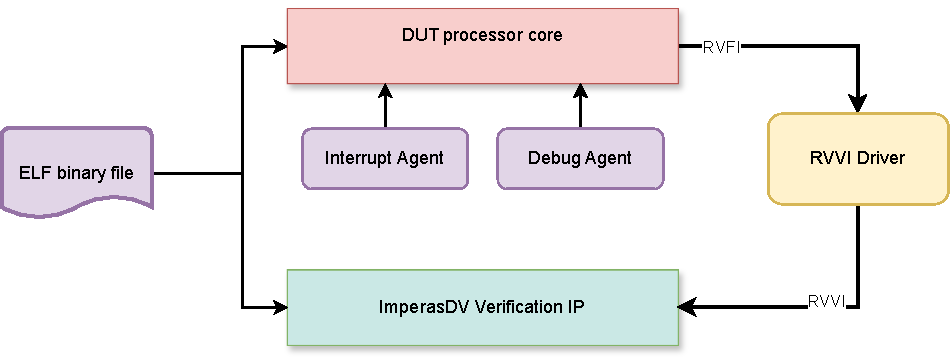
\includegraphics[width=0.75\linewidth]{figures/core-v-verif.pdf}
    \caption{Overview of the verification environment for the CV32E40S core based on figure from \cite{openhwgroupOpenhwgroupCorevverif2023}.}
    \label{fig:cv32e40s-overview}
\end{figure}


\subsection{RVFI - Risc-V Formal Interface}
\label{sec:rvfi}

The RVFI specification is an interface of output signals from the core and is used to compare the execution with the reference model. 
When an instruction is retired from the core, it asserts the \lstinline{rvfi_valid} signal and outputs the details of the retired instruction and updates to GPR, CSR, PC, etc. \cite{symbioticedaRiscvformalDocsRvfi2020}.

RVFI also supports reporting of asynchronous events out from the core. In RVFI, interrupts are reported as happening between instructions, so the results from the interrupt will be shown in the first instruction of the trap handler by asserting the \lstinline{rvfi_intr} signals to indicate the interrupt type and cause \cite{openhwgroupRISCVFormalInterface2023}.

This allows the interrupt and debug generators to be connected only to the DUT and the reference model to be alerted of interrupts when reported through the DUT.
This ensures the timing of interrupts stays in sync in the DUT and reference model. However, this also results in the reference model being unable to verify if the DUT takes the interrupts correctly, for instance, when multiple interrupts are present simultaneously \cite{taylorAdvancedRISCVVerification2023}.

%The full list of RVFI signals for the CV32E40S core can be found in \cite{openhw_group_risc-v_2023}, but some useful signals are listed below.
%
%\begin{itemize}
%    \item \lstinline{rvfi_insn} - The retired instruction word
%    \item \lstinline{rvfi_trap} - Signals that a synchronous trap has occurred, like a trap, exception, debug, etc.
%    \item \lstinline{rvfi_intr} - Signals that an interrupt has occurred, with the cause.
%    \item \lstinline{rvfi_pc_rdata} - PC of the retired instruction
%    \item \lstinline{rvfi_pc_wdata} - Next predicted PC. Ignores asynchronous traps
%    \item \lstinline{rvfi_csr_...} - Control and status register
%    \item \lstinline{rvfi_gpr_...} - The general purpose registers (x0-x31)
%    
%\end{itemize}



\subsection{RVVI - RISC-V Verification Interface}
\label{sec:rvvi}

RVVI is an open verification interface used to connect the DUT and reference model. 

The RVVI-API is a set of functions implemented in the reference model and testbench to generalize the communication with the reference model, making it easier to replace. It has functions for configuring the model, stepping, and passing asynchronous events, etc. \cite{riscv-verificationRISCVVerificationInterface2023}.

Interrupts can be passed to the reference model using \lstinline{rvviRefNetSet(netIndex, value, when)} to set signals at a specific clock cycle \cite{riscv-verificationRISCVVerificationInterface2023}.


%There are lots of conditions for interrupts that must be taken into consideration. Here are some example conditions from \lstinline{ev32e40x_controller_fsm.sv} from the cv32e40x core:
%\begin{itemize}
%    \item When an interrupt is pending, and can not be taken immediately, the ID stage is halted
%    \item Interrupts can only be taken if there is no data request in WB, and no trans\_valid has been clocked from EX to environment.
%    \item Interrupts can not happen if multi-cycle operations are in WB
%    \item If a clic pointer is in EX or WB, we must block interrupts
%\end{itemize}

% \url{https://www.youtube.com/watch?v=iQR_6f5Jdns}
%Exceptions can happen in any pipeline stage, e.g. memory faults in IF and MEM stages, Illegal instructions in ID, Arithmetic exceptions in ALU, etc. 
%
%When exceptions happen, the instructions following the instruction causing the exception need to be discarded. Since register values are only updated in the WB stage, annulling can be done by replacing the instruction with NOP.
%Exceptions can be thought of as implicit branches, that branch to the exception handler.
%
%Interrupts are also implicit branches. External interrupts can be handled as exceptions that affect the IF stage. The instruction in IF when the interrupt happens is replaced with BNE and the next instruction is the address of the interrupt handler.




%from \lstinline{cv32e40x}: 
%
%\begin{lstlisting}
%    // In addition the ID stage may be halted to enable interrupts or debug to be taken.
%    //   - If an interrupt (including NMI) is present it is not guaranteed that the pipeline
%    //     can take the interrupt immediately. A \acrshort{lsu} instruction could for instance be outstanding, causing the interrupt not to be taken.
%    //     The controller uses (pending_interrupt && interrupt_allowed) to check for these conditions.
%    //     When an interrupt (or NMI) is pending, the ID stage is halted to guarantee that an interruptible bubble eventually will
%    //     occur in the WB stage.
%    //   -- The ID stage is only halted iff debug_interruptible==1, indicating that we are not in debug mode or single step mode with interrupts disabled.
%    //   --- If halting for interrupts while in debug mode (debug_interruptible == 0), the core would deadlock waiting for interrupt_allowed, but the core
%    //       would never exit debug mode because the dret instruction could be blocked by the halted ID stage.
%    //   -- The ID stage is only halted iff also the ID stage is haltable (meaning ID stage is not currently in the middle of a sequence or waiting for a CLIC pointer)
%    //
%    //   - The ID stage is halted when any async or sync debug is pending for the same reasons as for interrupts.
%    //
%    //   - If not checking for id_stage_haltable for interrupts and debug, the core could end up in a situation where it tries to create a bubble
%    //     by halting ID, but the condition disallowing interrupt or debug will not disappear until the sequence currently handled by the ID stage
%    //     is done. This would create an unrecoverable deadlock.
%\end{lstlisting}
%
%\begin{lstlisting}
%  // Allow interrupts to be taken only if there is no data request in WB,
%  // and no trans_valid has been clocked from EX to environment.
%  // Not allowing interrupts when the core cannot take interrupts due to debug conditions.
%  // Offloaded instructions in WB also block, as they cannot be killed after commit_kill=0 (EX stage)
%  // \acrshort{lsu} instructions which were suppressed due to previous exceptions or trigger match
%  // will be interruptable as they were converted to NOP in ID stage.
%  // When a fencei is present in WB and the \acrshort{lsu} has completed all tranfers, the fencei handshake will be initiated. This must complete and the fencei instruction must retire before allowing interrupts.
%  // Any multi operation instruction (table jumps, push/pop and double moves) may not be interrupted once the first operation has completed its operation in WB.
%  //   - This is guarded with using the sequence_interruptible, which tracks sequence progress through the WB stage.
%  // When a CLIC pointer is in the pipeline stages EX or WB, we must block interrupts.
%  //   - Interrupt would otherwise kill the pointer and use the address of the pointer for mepc. A following mret would then return to the mtvt table, losing program progress. 
%\end{lstlisting}


\subsection{Virtual Registers}

\tmp{Describe the core-v-verif virtual registers}







\section{The problem with using an ISS as a reference model}
\label{sec:back_issProblem}

All the implementations from \cref{sec:bg_existingReference} except ImperasDV uses an ISS as a reference model. \textcite{taylorAdvancedRISCVVerification2023}  discuss multiple problems when using an ISS as a reference model. The first problem is the difference in abstraction level between the DUT and the ISS. On one hand, the DUT is typically simulated at a clock-cycle accurate Register Transfer Level. On the other hand, ISSs are simulated with time modeled at the instruction level, with the cycle timing of memory interfaces and pipeline operation abstracted away. This leads to an inconsistency between the two. For instance, the RTL model might take multiple clock cycles to complete an instruction while the ISS executes it in one cycle.

When there are no asynchronous events, the ISS can accurately predict the execution of instructions. The problem arises with asynchronous events. In an instruction-accurate simulator, interrupts and debug requests are seen as happening at the beginning of a new instruction, while in the DUT, they could happen in the middle of a multi-cycle instruction. In addition, the ISS does not know the state of the pipeline. In some cases, as explained in \cref{sec:bg_pipeline}, the pipeline has states where interrupts can not immediately be taken, causing a mismatch where the ISS takes the interrupt before the DUT.



Another problem discussed is the timing of \textit{side effects}, which are state changes not explicitly part of the instruction \cite{taylorAdvancedRISCVVerification2023}. Typically, this can be predicted with an ISS in normal execution, but they can be inaccurate when asynchronous interrupts are introduced, where the pipeline execution can alter the timing of the side effects.

\tmp{Expand this with examples}

\tmp{Should this be moved outside of background and use more custom examples?}

%This has typically been done with the "step-and-compare" methodology, where the DUT runs until an instruction retires, then the RTL clock is stopped and the reference model is run until it also retires an instruction. At this point, the testbench compares the states in the DUT and RM before starting the RTL clock again.

\section{Cycle-accurate modeling techniques}
\label{sec:bg_cycle-accurate}

Multiple approaches for cycle-accurate modeling have previously been attempted for different processors and instruction set architectures.

Chiang and Huang proposed a two-layered cycle-accurate modeling technique that partitions the simulator into an untimed functional kernel and an outer timing shell. The inner functional kernel is essentially an untimed ISS responsible for executing the instruction and calculating the correct register values, outputs, and memory data \cite{chiangEfficientTwolayeredCycleaccurate2009}.

The timing shell is shown in \cref{fig:timeshell}, sits on top of the functional kernel, interacts with the rest of the system, and updates the changes calculated in the functional kernel at the correct time. The timing shell consists of a commander that takes in external inputs, checks the internal processor state, and determines whether there should be a stall. If the processor should not stall, the commander either sends a \textit{step} or \textit{interrupt} command to the functional unit according to the inputs and receives a result packet when the functional unit has completed. The result goes into the scheduler, which correctly times the updates from the result packet to the right clock cycle in the time wheel described below. To place updates correctly into the time wheel, the scheduler needs to know all the implementation details of the processor. This includes what happens in each pipeline stage, dependencies between instructions, instruction cycle timing, hazard detection, and stall/forwarding functionality. \cite{chiangEfficientTwolayeredCycleaccurate2009}


The time wheel consists of multiple time slots corresponding to specific clock cycles and holds all the data to update the outputs and registers at the correct clock cycle. Because of the processor pipeline, one instruction might need to update multiple time slots if the instruction has side effects in different stages. It also has a field indicating if the cycle should stall or not, in which case no command packet is sent to the functional kernel. The time wheel advances each clock cycle, and the most recent time slot is executed.

Another cycle-accurate is the FaCSim, a fast and cycle-accurate architecture simulator by Lee et al. that follows a strategy similar to Chiang and Huang's. FaCSim also consists of a functional simulator and a Cycle-Accurate Trace simulator with a slightly different approach. The functional simulator is responsible for fetching instructions from the ELF executable, decoding, and executing it. It generates an execution trace that is stored in a circular queue connecting the functional simulator and cycle-accurate simulator. \cite{leeFaCSimFastCycleAccurate2008}

The execution trace consists of the fetched instruction, the EX stage execution latency, memory traces, etc. The functional simulator also keeps track of pipeline interlocks and simulates stalls by inserting empty bubble instruction trances to simulate stalls from hazards and branches \cite{leeFaCSimFastCycleAccurate2008}.

Instead of performing cycle-by-cycle instructions simulation, the simulator computes the elapsed cycle in each stage of the pipeline and adds them up to advance the clock. 

The cycle-accurate simulator loads instruction traces from the circular queue and makes it go through the pipeline. Each pipeline stage has a corresponding function that calculates the delay for each stage. After the delay has been calculated for all stages, the core clock is updated after the writeback stage. 
\cite{leeFaCSimFastCycleAccurate2008}

\begin{figure}[htb]
    \centering
    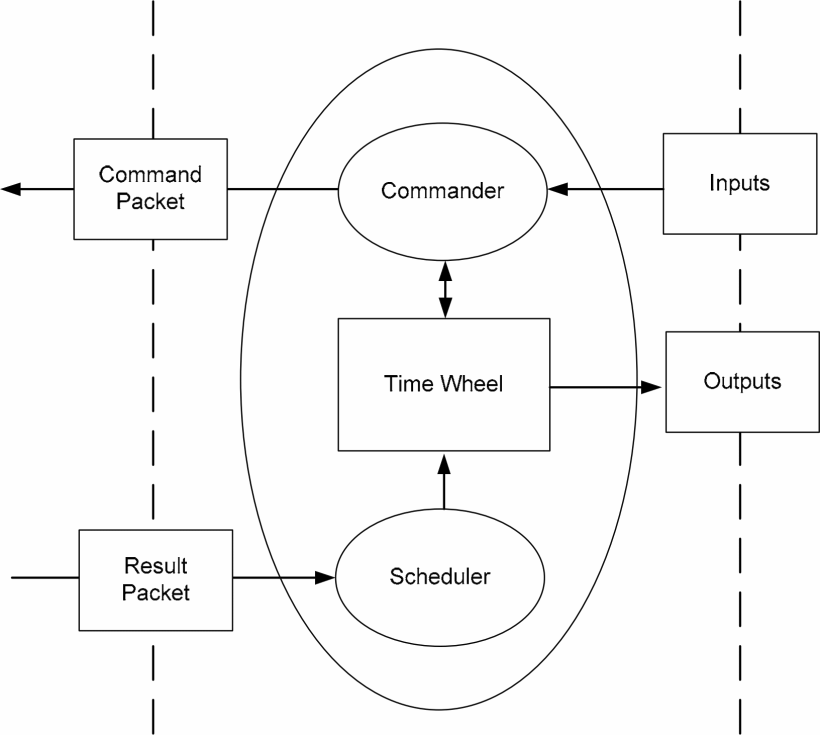
\includegraphics[width=0.5\linewidth]{figures/timeShell.png}
    \caption{Architecture of the timing shell from \cite{chiangEfficientTwolayeredCycleaccurate2009}.}
    \label{fig:timeshell}
\end{figure}
%\section{Pipeline simulation approaches}
%
%Poroshin, P.A., and A.N. Meshkov. propose several approaches to pipeline simulation for turning an ISS into a cycle-accurate simulator in \cite{poroshin_exploration_2019}. They are making a simulator for the "Elbrus" VLIW ISA, but some of the principles are still relevant for a RISC-V reference model.  One difference is that their cycle-accurate simulator is focused on debugging performance problems and not verification, so some principles might not be applicable. They describe the following pipeline models:
%
%\subsection{Naive "Direct Correspondence" Pipeline Model }
%
%In the Naive each pipeline phase is split into different functions which determine which instruction is at this stage and execute the functions depending on the instructions. 
%
%This approach is the most similar to the actual hardware but has some disadvantages. It requires modifying the original ISS by splitting it up into pieces and gluing them back together. This makes it harder to keep the ISS up to date. Keeping track of all pipeline stages also adds complexity and overhead.
%
%This is the only approach that handles the special case where timing behaviour influences the algorithmic behaviour. 
%\subsection{Smart "Direct Correspondence" Pipeline Model }
%
%The smart "Direct Correspondence" Pipeline Model is a modification of the Naive model, where the functional actions and timing actions are split. Here all the functional logic is moved to the beginning of the instruction processing and only the timing is simulated in the following pipeline stages.
%
%A similar approach is used in \cite{bohm_cycle-accurate_2010} to make a cycle-accurate performance model in a JIT DBT simulator. This is a fast cycle-accurate ISS for the ARCompact RISC (not RISCV) ISA. This also works by reconstructing the pipeline state after executing an instruction.
%
%\subsection{"Fully Speculative" Pipeline model}
%
%Simulates the entire instruction in one go before considering the next instructions. 
%
%Will be complicated to do in lock-step execution.
%
%
%\subsection{Hybrid Pipeline model}
%
%A combination of smart "direct correspondence" and fully speculative


%\section{OBI}
%
%
%
%\section{ABI \& ELF}
%
%\url{https://www.youtube.com/watch?v=F2uIiOw8CfI}
%ABI Application Binary Interface
%
%interface between application program and operating system
%a set of conventions
%
%RISCV ilp32
%
%\begin{table}
%    \centering
%    \begin{tabular}{ccc}
%        Register & ABI name & Description\\
%        x0 & zero & Hard-wired zero\\
%        x1 & ra & Return address\\
%        x2 & sp & stack pointer\\
%        ... & ... & ...\\
%    \end{tabular}
%    \caption{Caption}
%    \label{tab:my_label}
%\end{table}

%\subsection{ELF Executable and linkable format}
%
%\begin{itemize}
%    \item Agnostic to a processor, instruction set, hardware and OS
%    \item Consists of ELF header and file data
%\end{itemize}
%
%
%\textbf{Header} can contain start address and other info 
%
%\textbf{Sections} hold information required for linking the object files
%
%only required during link time and not run time
%
%\textbf{Program headers or segments}
%
%break down elf binary into suitable chunks to prepare the executable to be loaded into memory
%
%OS would parse the information in the header and determine where to load each section
%
%\textbf{Loader loads elf into memory}
%
%bare metal uses static linking
%
%bare metal vs os
%
%os does memory management etc. printf etc.
%
%bare metal: must have a minimal implementation of printf in the program

\section{Formal Verification}

\tmp{TODO: Må jeg ha med SVA?}

\tmp{TODO: expand and rewrite}

Formal verification is using mathematical tools to analyze the space of possible behaviors of a design \cite{seligmanFormalVerificationEssential2015}.

Validating a design requires a \textit{specification} and an \textit{implementation}. The specification is often a more abstract description of the design requirements in the form of properties like \acrfull{sva}, an \acrshort{rtl} model, or a high-level model\cite[p. 26]{seligmanFormalVerificationEssential2015}. 

\section{Advantages}

\begin{itemize}
    \item Complete coverage
    \item Minimal examples, not a part of 10000 cycles of random instructions
\end{itemize}



\subsection{Model Checking}

\textit{Model checking} is a widely used \acrshort{fv} technique that analyses the behavior of a system over a period of time. It can search over the possible future states of a model and check if defined properties are violated or not \cite{seligmanFormalVerificationEssential2015}. One challenge with model checking is to determine a set of properties that fully covers the behavior of the model without being redundant and covering every corner case \cite{castromarquezFormalEquivalenceChecking2013}.

\section{Formal Equivalence Verification}

\acrfull{fev} is a formal verification tool that compares the RTL code to a reference model \cite{seligmanFormalVerificationEssential2015}.

The most common usecases are \acrshort{rtl} to netlist \acrshort{fev} or \acrshort{rtl} to \acrshort{rtl} \acrshort{fev}

\subsection{Sequential Equivalence}

Verifies if two models will generate the same result after the same time with equal inputs. The internal state elements does not have to be identical, only the outputs \cite{seligmanFormalVerificationEssential2015}.

If sequential \acrshort{fev} tools are available \textcite{seligmanFormalVerificationEssential2015} recommends using these tools instead of writing properties if the reference model is complete enough.

Requirements for sequential \acrshort{fev} is:
\begin{itemize}
    \item RTL model
    \item Mature tools
\end{itemize}


%Possible approaches:
%\begin{itemize}
%    \item High-level Model Equivalence Verification \cite{seligmanFormalVerificationEssential2015}. "Modeling in a language more abstract than RTL, such as SystemC has been used at intel, but lack good commercial EDA support"
%    \item Express specifications as properties \cite{piskacEndtoEndFormalVerification2021}
%\end{itemize}



\section{Tools}

\subsection{Jasper Gold}
The Jasper Sequential Equivalence Checking (SEC) App \footnote{\url{https://www.cadence.com/en_US/home/tools/system-design-and-verification/formal-and-static-verification/jasper-gold-verification-platform/jaspergold-sequential-equivalence-checking-app.html}}
is a formal verification tool that allows sequential equivalence checking of two \acrshort{rtl} models.

Can verify the sequential equivalence of two RTL models.

Mostly used to verify:
\begin{itemize}
    \item Small changes
    \item Two different implementations
    \item Optimizations
    \item Proove backwards compatibility
    \item Comparing two different implementations
\end{itemize}

\subsection{Onespin}

\tmp{TODO: Explain onespin}

360 EC-RTL \footnote{\url{https://www.onespin.com/products/360-ec-rtl}}

360 EC-FPGA also has sequential equivalence checking

\begin{itemize}
    \item Comparison of two RTL blocks.
    \item Hard to find open documentation
\end{itemize}


\subsection{Limitations}

\begin{itemize}
    \item Can these tools handle the large scale of a full core, or are they meant to handle smaller modules?
    \item Do they work with SystemVerilog generated from the sail-riscv model?
\end{itemize}

For \acrshort{fev}
\begin{itemize}
    \item Both RTL models have to be fully behaviorally equivalent.
    \item Must be fully cycle-accurate equivalent (Not only comparable at retirement)
\end{itemize}
